\documentclass[11pt,aspectratio=169]{beamer}
%\documentclass[11pt,aspectratio=169,handout]{beamer}

\usepackage{amsmath}
\usepackage{amsfonts}
\usepackage{amssymb}
\usepackage{graphbox}
\usepackage{sgamevar}
\usepackage{pgfplots}
\usepackage{tikz}
\usepackage{pstricks,pst-node}
\usepackage{bigdelim}
\usepackage{qrcode}
\usepackage{dsfont}
\usepackage[absolute,overlay]{textpos}
\usepackage[ruled,vlined]{algorithm2e}



% alg
\SetKwFor{Repeat}{repeat}{}{}
\SetKwComment{Comment}{$\triangleright$ }{}
\SetCommentSty{textsf}
% pgfplot settings
\usepgfplotslibrary{fillbetween}

% tikz settings
\tikzset{
    invisible/.style={text opacity=1,opacity=0},
    visible on/.style={alt=#1{}{invisible}},
    alt/.code args={<#1>#2#3}{%
      \alt<#1>{\pgfkeysalso{#2}}{\pgfkeysalso{#3}}
    },
  }
\newcommand{\nebox}[2][]{\tikz[baseline=(h.base)]\node[rounded corners,rectangle,draw,line width=0.7pt,text depth=-4.9pt,#1] (h) {#2};}
\usetikzlibrary{arrows}
% Customized colors

\definecolor{ashgrey}{rgb}{0.7, 0.75, 0.71}
\definecolor{lightblue}{RGB}{140, 201, 247}
\definecolor{darkgreen}{RGB}{113, 160, 55}
\definecolor{darkblue}{RGB}{78, 103, 200}
\definecolor{darkpurple}{RGB}{112, 48, 160}
\definecolor{xgray}{rgb}{0.75, 0.75, 0.75}
\definecolor{lightgreen}{rgb}{0.56, 0.93, 0.56}

% Hyperlink settings

\hypersetup{colorlinks,urlcolor=darkgreen}

%Beamer settings

\setbeamertemplate{navigation symbols}{} 
\setbeamertemplate{footline}[frame number]
\setbeamertemplate{itemize items}[circle]
\setbeamertemplate{section in toc}[sections numbered]
\setbeamertemplate{subsection in toc}[subsection numbered]

\setbeamercolor{section in toc}{fg=blue}

\AtBeginSection[ ]{
 \begin{frame}{Outline}
  \hypersetup{linkcolor=black}
  \tableofcontents[currentsection]
 \end{frame}
}

% Graphics settings

\graphicspath{{../Figures/}}

% PGFPlot settings

\pgfplotsset{compat = newest}

% Gamesvar settings

\setlength{\arrayrulewidth}{0.91pt}
\renewcommand{\gamestretch}{1.68}
\def\stackedpayoffs#1#2{%
 \begin{array}{c}#1\\[2mm]#2\end{array}
}

% Math

\DeclareMathOperator*{\argmax}{argmax}
\DeclareMathOperator*{\argmin}{argmin}
\DeclareMathOperator{\E}{\mathbb{E}}

\newcommand\given[1][]{\:#1\vert\:}
\newtheorem{proposition}{Proposition}
\newcommand{\OPT}{{\rm OPT}}

% New environments

\newenvironment{itemizes}[1][1em]{
 \vspace{#1}
 \begin{itemize}
 \setlength{\itemsep}{#1}
}{
 \end{itemize}
}


% Shared title frame

\title{Game-theoretic \\ Foundations of Multi-agent Systems}

\author{Seyed Majid Zahedi}
\titlegraphic{\vspace{-4.2em} 
\includegraphics[height=5.8em]{Logos/logo2}}

\date{} 
\subject{Lecture 1} 
\logo{\includegraphics[height=5.6em]{Logos/logo1}}
\subtitle{\vspace{2.1em}Lecture 7: Stochastic Games}

\begin{document}

 \begin{frame}[plain]
  \titlepage
 \end{frame}
 
 
 \section{Markov Decision Processes}
 
  \begin{frame}{Motivation: Non-deterministic Search in Grid World}
   \begin{center}
    \includegraphics[width=0.7\textwidth]{L7/Motivation}
   \end{center}
  \end{frame}
  
  
  \begin{frame}{Grid World Actions}
   \begin{columns}
    \begin{column}{0.3\textwidth}
     \begin{center}
      \textbf{Deterministic}
     \end{center}
     \vspace{0.05cm}
     \begin{center}
      \includegraphics[width=0.5\textwidth]{L7/Deterministic}
     \end{center}
    \end{column}
    \begin{column}{0.7\textwidth}
     \visible<2->{
      \begin{center}
       \textbf{Stochastic}
      \end{center}
      \vspace{0.1cm}
      \begin{center}
       \includegraphics[width=0.65\textwidth]{L7/Stochastic}
      \end{center}
     }
    \end{column}
   \end{columns}
  \end{frame}
  
  
  \begin{frame}{A Grid World Instance}
   \begin{columns}
    \begin{column}{0.6\textwidth}
     \begin{itemize}
     \setlength{\itemsep}{0.5em}
      \item Agent lives in a grid
      \item Walls block agent's path
      \item Actions do not always go as planned
      \begin{itemize}
       \item 80\% of time, action ``North'' takes us north
       \item 10\% of time, ``North'' takes us west; 10\% east
       \item If there is a wall in the direction the agent would have been taken, the agent stays put
      \end{itemize}
      \item Agent receives rewards at each step
      \item Goal is to maximize sum of rewards
     \end{itemize}
    \end{column}
    \begin{column}{0.4\textwidth}
     \begin{center}
      \includegraphics[width=0.9\textwidth]{L7/Search}
     \end{center}
    \end{column}
   \end{columns}
  \end{frame}
  
  
  \begin{frame}{Change in Notation}
   \begin{itemizes}[2em]
    \item So far, we have used \alert{$s$} to denote \alert{strategy profile}
    \item In this lecture, we use \alert{$\pi$} for strategy
    \item We use \alert{$s$} to denote \alert{state}
   \end{itemizes}
  \end{frame}
  
  
  \begin{frame}{Markov Property}
   \begin{textblock*}{3cm}(12cm,1cm)
    \begin{center}\tiny
     \includegraphics[width=0.85\textwidth]{L7/Markov}
     \vspace{5pt}
     Andrey Markov (1856-1922)
    \end{center}
   \end{textblock*}
   \vspace{40pt}
   \begin{itemize}
   \setlength{\itemsep}{2em}
    \item<+-> Given present state, future and past are independent
    \item<+-> Future state depends only on current state and action
    \vspace{10pt}
    \visible<+->{
     \begin{align*}
      P(S_{t+1}=s &\given S_t=s_t, A_t=a_t, S_{t-1}=s_{t-1}, A_{t-1}=a_{t-1}, \dots, S_0 = s_0) = \\
      P(S_{t+1}=s &\given S_t=s_t, A_t=a_t)
     \end{align*}
    }
   \end{itemize}
  \end{frame}
  
  
  \begin{frame}{Markov Decision Processes: Formal Definition}
   \begin{columns}
    \begin{column}{0.7\textwidth}
     \begin{itemize}
     \setlength{\itemsep}{1em}
      \item<+-> $S$ is set of states and $A$ is set of actions
      \item<+-> $p: S \times A \times S \mapsto [0,1]$ specifies transition probabilities
      \vspace{5pt}
      \begin{itemize}[<.->]
       \item $p(s, a, s^\prime)$ is probability of going to $s^\prime$ when taking $a$ in $s$
      \end{itemize}
      \item<+-> $r: S \times A \times S \mapsto \mathbb{R}$ returns reward
      \vspace{5pt}
      \begin{itemize}[<.->]
       \item $r(s, a, s^\prime)$ is reward of going to $s^\prime$ when taking $a$ in $s$
      \end{itemize}
      \item<+-> There are two ways to aggregate rewards
      \begin{itemizes}
       \item Limit-average reward: $\lim_{T\rightarrow\infty}\sum_{t=1}^{T}r_t/T$
       \item \alert<+->{Future-discounted reward: $\sum_{t=1}^{\infty}\delta^{t-1} r_t$} \\
       \visible<+->{(we will focus on this)}
      \end{itemizes}
     \end{itemize}
    \end{column}
    \begin{column}{0.3\textwidth}
     \begin{center}
      \includegraphics<1->[width=0.85\textwidth]{L7/Grid}
     \end{center}
    \end{column}
   \end{columns}
  \end{frame}
  
  
  \begin{frame}{Example: Racing}
   \begin{itemize}
    \item Autonomous car wants to travel far, quickly
    \item There are 3 states: Cool, Warm, Overheated, and 2 actions: {\color{blue} Slow}, {\color{red}Fast}
    \item Going faster gets double reward
   \end{itemize}
   \vspace{10pt}
   \begin{center}
    \includegraphics[width=0.7\textwidth]{L7/Cars}
   \end{center}
  \end{frame}
  
  
  \begin{frame}{Policies}
   \begin{columns}
    \begin{column}{0.6\textwidth}
     \begin{itemize}
     \setlength{\itemsep}{1.2em}
      \item A \alert{(stationary, deterministic)} policy $\pi: S \mapsto A$ gives action for each state
      \item An \alert{optimal} policy is one that maximizes expected utility if followed
     \end{itemize}
    \end{column}
    \begin{column}{0.4\textwidth}
     \begin{center}\scriptsize
      \includegraphics[width=0.9\textwidth]{L7/Policies}
     \end{center}
    \end{column}
   \end{columns}
  \end{frame}
  
  
  \begin{frame}{Values of States}
   \begin{itemize}[<+->]
   \setlength{\itemsep}{1em}
    \item \alert{Value function}: $V^\pi(s)$ specifies value of following $\pi$ starting in $s$
    $$V^\pi(s)=\mathbb{E}\left[\sum_{t=1}^{\infty}\delta^{t-1}r_t(s_t, \pi(s_t), s_{t+1}) \given s_0 = s\right]$$
    \item \alert{State-action value function}: $Q^\pi(s,a)$ returns value of starting in $s$, taking $a$, and then continuing according to $\pi$
    \item These two are related to each other by
    \begin{align*}
     &Q^\pi(s,a) = \sum_{s^\prime}p(s, a, s^\prime) \left(r(s, a, s^\prime) + \delta V^\pi(s^\prime)\right) \\
     &V^\pi(s) = Q^\pi(s, \pi(s)) \\[0.5em]
     \visible<4->{\Rightarrow \;\; &V^\pi(s) = \sum_{s^\prime}p(s, \pi(s), s^\prime) \left(r(s, \pi(s), s^\prime) + \delta V^\pi(s^\prime)\right)}
    \end{align*}
   \end{itemize}
  \end{frame}
  
  
  \begin{frame}{Policy Evaluation}
   \begin{algorithm*}[H]
    Initialize $V^\pi_{0}(s)$ $\leftarrow$ 0 for all states $s$\;
    \For{$t = 1 \dots T$}{
     \For{each state $s$}{
      $V^\pi_{t}(s) \leftarrow \sum_{s^\prime}p(s, \pi(s), s^\prime) \left(r(s, \pi(s), s^\prime) + \delta V^\pi_{t-1}(s^\prime)\right)$
     }
    }
   \end{algorithm*}
   \vspace{0.7cm}
   \begin{itemize}[<+->]
    \item How many iterations should we have (what should $T$ be)?
    \item Repeat until values do not change much:
    $$\underset{s\in S}{\max} \;\; \vert V^\pi_{t}(s) - V^\pi_{t-1}(s) \vert < \epsilon$$
   \end{itemize}
  \end{frame}
  
  
  \begin{frame}{Solving MDP: Bellman Equations}
   \begin{align*}
     &Q^*(s,a) = \sum_{s^\prime}p(s, a, s^\prime) \left(r(s, a, s^\prime) + \delta V^*(s^\prime)\right) \\[1em]
     &V^*(s) = \underset{a\in A}{\max} \;\; Q^*(s, a) \\[1em]
     \Rightarrow \;\; &V^*(s) = \underset{a\in A}{\max} \;\; \sum_{s^\prime}p(s, a, s^\prime) \left(r(s, a, s^\prime) + \delta V^*(s^\prime)\right)
   \end{align*}
  \end{frame}
  
  
  \begin{frame}{Value Iteration}
   \begin{algorithm*}[H]
    Initialize $V_{0}(s)$ $\leftarrow$ 0 for all states $s$\;
    \Repeat{until $V(s)$ converges for all $s$}{
     \For{each state $s$}{
      $V_{t}(s) \leftarrow \underset{a\in A}{\max} \;\; \sum_{s^\prime}p(s, a, s^\prime) \left(r(s, a, s^\prime) + \delta V_{t-1}(s^\prime)\right)$
     }
    }
   \end{algorithm*}
   \vspace{0.5cm}
   \begin{itemize}
    \item<2-> Bellman equations \alert{characterize} the optimal values
    \item<3-> Value iteration \alert{computes} them
    \item<4-> Value iteration is just a \alert{fixed-point} solution method
   \end{itemize}
  \end{frame}
  
  
  \begin{frame}{Policy Extraction}
   \begin{itemize}[<+->]
    \item Given $V^*$, we can compute optimal policy as follows:
    $$\pi^*(s) = \underset{a}{\argmax} \;\; \sum_{s^\prime}p(s, a, s^\prime) \left(r(s, a, s^\prime) + \delta V^*(s^\prime)\right)$$
    \item Given $Q^*$, we can compute optimal policy as follows:
    $$\pi^*(s) = \underset{a}{\argmax} \;\; Q^*(s, a)$$
    \item Takeaway: actions are easier to select from Q-values than values!
   \end{itemize}
  \end{frame}
  
  
  \begin{frame}{Problems with Value Iteration}
   \begin{itemizes}[1.5em]
    \item It is slow - $O(S^2 A)$
    \item The $\max$ at each state rarely changes
    \item The policy often converges long before the values
   \end{itemizes}
  \end{frame}
  
  
  \begin{frame}{Policy Iteration}
   \begin{columns}
    \begin{column}{0.75\textwidth}
     \begin{itemize}[<+->]
     \setlength{\itemsep}{1.2em}
      \item \alert{(I) Policy evaluation:} Calculate values for some fixed policy
      \item \alert{(II) Policy improvement:} Extract policy given these values
      \item Repeat steps until policy converges
     \end{itemize}
    \end{column}
    \begin{column}{0.25\textwidth}
     \begin{center}
      \includegraphics<1->[width=0.9\textwidth]{L7/PI}
     \end{center}
    \end{column}
   \end{columns}
  \end{frame}
  
  
  \begin{frame}{Value Iteration vs Policy Iteration}
   \begin{itemize}[<+->]
   \setlength{\itemsep}{1em}
    \item Both compute the same thing (all optimal values)
    \item In \alert{value iteration:}
    \begin{itemize}
     \item Every iteration updates both values and (implicitly) policy
     \item We don't track policy, but taking $\max$ over actions implicitly recomputes it
    \end{itemize}
    \item In \alert{policy iteration:}
    \begin{itemize}
     \item We do several passes that update values with fixed policy\\(each pass is fast because we consider only one action, not all of them)
     \item After policy is evaluated, a new policy is chosen\\(slow like a value iteration pass)
     \item New policy will be better (or we're done)
    \end{itemize}
    \item Both are \alert{dynamic programs} for solving MDPs
   \end{itemize}
  \end{frame}
  
  
 \section{Definition of Stochastic Games}
 
  \begin{frame}{Stochastic Games (a.k.a. Markov Games): Introduction}
   \begin{textblock*}{3cm}(12cm,2.5cm)
    \begin{center}\tiny
     \includegraphics[width=0.85\textwidth]{L7/Shapley}
     \vspace{5pt}
     Lloyd Shapley (1923-2016)
    \end{center}
   \end{textblock*}
   \vspace{2em}
   \begin{itemize}[<+->]
   \setlength{\itemsep}{1em}
    \item Lloyd Shapley introduced stochastic games in early 1950s
    \item Stochastic games generalize repeated games
    \begin{itemize}
     \item Agents repeatedly play games from set of stage games
    \end{itemize}
    \item Stochastic games generalize Markov decision process
    \begin{itemize}
     \item Game at each step only depends on outcome of previous step
    \end{itemize}
    \item \alert{Single-state} stochastic game = (infinitely) repeated game
    \item \alert{Single-agent} stochastic game = MDP
   \end{itemize}
  \end{frame}
  
  
  \begin{frame}{Repeated Games vs Stochastic Games}
   \begin{columns}
    \begin{column}{0.4\textwidth}
     \visible<1->{\begin{center} \vspace{-8em}
      \textbf{Repeated Games} \\ \vspace{2em}
      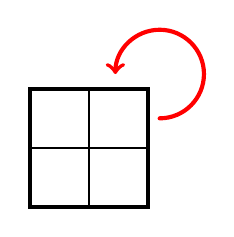
\begin{tikzpicture}[x=0.75cm,y=0.75cm]
       \draw[black, thick, line width=1.5pt, line cap=rect] (0,0) -- (0, -2);
       \draw[black, thick] (1,0) -- (1, -2);
       \draw[black, thick, line width=1.5pt, line cap=rect] (2,0) -- (2, -2);
       \draw[black, thick, line width=1.5pt, line cap=rect] (0,0) -- (2, 0);
       \draw[black, thick] (0,-1) -- (2, -1);
       \draw[black, thick, line width=1.5pt, line cap=rect] (0,-2) -- (2, -2);     
       \draw[red, thick, ->, line width=1.5pt, line cap=round] (2.2,-0.5) arc (-90:180:0.75);
      \end{tikzpicture}
     \end{center}}
    \end{column}
    \begin{column}{0.6\textwidth}
     \visible<2->{\begin{center}
      \textbf{Stochastic Games} \\ \vspace{2em}
      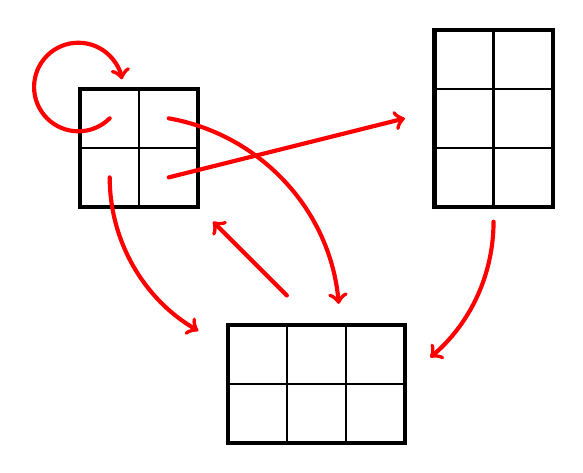
\begin{tikzpicture}[x=0.75cm,y=0.75cm]
       \draw[black, thick, line width=1.5pt, line cap=rect] (0,0) -- (0, -2);
       \draw[black, thick] (1,0) -- (1, -2);
       \draw[black, thick, line width=1.5pt, line cap=rect] (2,0) -- (2, -2);
       \draw[black, thick, line width=1.5pt, line cap=rect] (0,0) -- (2, 0);
       \draw[black, thick] (0,-1) -- (2, -1);
       \draw[black, thick, line width=1.5pt, line cap=rect] (0,-2) -- (2, -2);
       
       \draw[red, thick, ->, line width=1.5pt, line cap=round] (0.5,-0.5) arc (-45:-350:0.75);
       \draw[red, thick, ->, line width=1.5pt, line cap=round] (1.5,-0.5) arc (80:5:3.5);
       \draw[red, thick, ->, line width=1.5pt, line cap=round] (0.5,-1.5) arc (180:240:3);
       \draw[red, thick, ->, line width=1.5pt, line cap=round] (1.5,-1.5) -- (5.5, -0.5);
       \draw[red, thick, ->, line width=1.5pt, line cap=round] (3.5,-3.5) -- (2.25, -2.25);
       \draw[red, thick, ->, line width=1.5pt, line cap=round] (7,-2.25) arc (0:-50:3);
              
       \draw[black, thick, line width=1.5pt, line cap=rect] (6,1) -- (6, -2);
       \draw[black, thick] (7,1) -- (7, -2);
       \draw[black, thick, line width=1.5pt, line cap=rect] (8,1) -- (8, -2);
       \draw[black, thick, line width=1.5pt, line cap=rect] (6,1) -- (8, 1);
       \draw[black, thick] (6,0) -- (8, 0);
       \draw[black, thick] (6,-1) -- (8, -1);
       \draw[black, thick, line width=1.5pt, line cap=rect] (6,-2) -- (8, -2);

       \draw[black, thick, line width=1.5pt, line cap=rect] (2.5,-4) -- (2.5, -6);
       \draw[black, thick] (3.5,-4) -- (3.5, -6);
       \draw[black, thick] (4.5,-4) -- (4.5, -6);
       \draw[black, thick, line width=1.5pt, line cap=rect] (5.5,-4) -- (5.5, -6);
       \draw[black, thick, line width=1.5pt, line cap=rect] (2.5,-4) -- (5.5, -4);
       \draw[black, thick] (2.5,-5) -- (5.5, -5);
       \draw[black, thick, line width=1.5pt, line cap=rect] (2.5,-6) -- (5.5, -6);
      \end{tikzpicture}
     \end{center}}
    \end{column}
   \end{columns}
  \end{frame}
  
  
  \begin{frame}{Stochastic Games: Formal Definition\footnotemark}
   \begin{itemizes}
    \item $S$ is finite set of \alert{stage games}
    \item $N$ is finite set of $n$ agents
    \item $A_i$ is finite set of actions available to agent $i$
    \item $p: S \times A \times S \mapsto [0,1]$ is \alert{transition probability function}
    \begin{itemize}
     \item $p(s,a,s^\prime)$ is probability of going from $s$ to $s^\prime$ after action profile $a$
    \end{itemize}
    \item $r_i: S \times A \mapsto \mathbb{R}$ is real-valued \alert{utility function} for agent $i$
    \begin{itemize}
     \item $r_i(s,a)$ is agent $i$'s utility at state $s$ for action profile $a$
    \end{itemize}
    \footnotetext[1]{\scriptsize Note that this definition assume actions available to agents are the same across different stage games. Changing this assumption leads to a more involved notation.}
   \end{itemizes}
  \end{frame}
  
  
 \section{Strategies and Equilibria in Stochastic Games}
 
  \begin{frame}{Stochastic Games: Strategies}
   \begin{itemize}
    \item Let $h_t =(s_0, a_0, s_1, a_1, \dots, a_{t-1}, s_t)$ denote \alert{history} of $t$ stages
    \item Let $H_t$ be set of all possible histories of this length
    \item Set of all \alert{deterministic} strategies for agent $i$ is
    $$\prod_{t,H_t}A_i$$
    \item Agents' strategies can consist of any mixture over deterministic strategies
    \item However, there are several restricted classes of strategies
   \end{itemize}
  \end{frame}
  
  
  \begin{frame}{Behavioral, Markov, and Stationary Strategies}
%  \small
   \begin{itemize}[<+->]
   \setlength{\itemsep}{1.2em}
    \item \alert{Behavioral} strategy $\pi_i(h_t, a_{i})$ returns probability of playing $a_i$ for $h_t$
    \begin{itemizes}[0.5em]
     \item<.-> Mixing takes place at each history independently
    \end{itemizes}
    \item \alert{Markov} strategy $\pi_i$ is behavioral strategy s.t. $\pi_i(h_t,a_i) = \pi_i(h^\prime_t,a_i)$ if $s_t = s_t^\prime$
    \begin{itemizes}[0.5em]
     \item<.-> $s_t$ and $s_t^\prime$ are final states of $h_t$ and $h^\prime_t$, respectively
     \item<.-> For each $t$, distribution over actions depends only on current state
    \end{itemizes}
    \item \alert{Stationary} strategy $\pi_i$ is a Markov strategy s.t. $\pi_i(h_{t_1}, a_i) = \pi_i(h^\prime_{t_2}, a_i)$ if $s_{t_1} = s^\prime_{t_2}$
    \vspace{0.5em}
    \begin{itemize}
    \setlength{\itemsep}{0.5em}
     \item<.-> $s_{t_1}$ and $s^\prime_{t_2}$ are final states of $h_{t_1}$ and $h^\prime_{t_2}$, respectively
     \item<.-> This removes possible dependence on time $t$
    \end{itemize}
   \end{itemize}
  \end{frame}
  
  
  \begin{frame}{Markov-perfect Equilibrium (MPE)}
   \begin{itemize}
   \setlength{\itemsep}{1.5em}
    \item Strategy $\pi$ is \alert{MPE} if it is Markov strategy and is NE regardless of starting state
    $$V_i^{\pi}(s) \ge V_i^{(\pi^\prime_i, \pi_{-i})}(s) \;\;\; \forall i, s, \pi_i^\prime$$
    \item MPE is similar to \alert{subgame-perfect equilibrium} in perfect-information games
    \item Every $n$-player, general-sum, \alert{discounted-reward} stochastic game has MPE
   \end{itemize}
  \end{frame}
  
  
  \begin{frame}{Computing Equilibrium}
   \begin{itemize}[<+->] 
   \setlength{\itemsep}{0.7em}
    \item Poly-time algorithms are not generally available for full class of stochastic games
    \item However, they exist for several nontrivial sub-classes
    \item E.g., 2-player, general-sum, discounted-reward, \alert{single-controller} stochastic games
    \begin{itemizes}[0.5em]
     \item<.-> Transitions depend on single agent: if $a_i = a^\prime_i$, then $p(s,a,s^\prime) = p(s,a^\prime,s^\prime)$ $\forall s, s^\prime$
    \end{itemizes}
    \item E.g., 2-player, general-sum, discounted-reward, \alert{separable-reward, state-independent-transition (SR-SIT)} stochastic games
    \begin{itemizes}[0.5em]
     \item<.-> $r_i(s, a) = f(s) + g(a)$ $\forall i, s, a$, and
     \item<.-> $p(s, a, s^{\prime\prime}) = p(s^\prime, a, s^{\prime\prime})$ $\forall s, s^\prime, s^{\prime\prime}, a$
    \end{itemizes}
    \item E.g., 2-player, zero-sum, discounted-reward stochastic games
   \end{itemize}
  \end{frame}
  
  
  \begin{frame}{Shapley Algorithm: Finding MPE in 2-player Zero-sum Games}
   \begin{algorithm*}[H]
    Initialize $V_0(s)$ arbitrarily for all $s$\Comment*{Agent 1's utility for being in $s$}
    \Repeat{until $V(s)$ converges for all $s$}{
     \For{each state $s$}{
      Compute matrix game $G(s,V_{t-1})$:
      $u(s, a) = r(s, a) + \delta \sum_{s^\prime}p(s, a, s^\prime)V_{t-1}(s^\prime)$
     }
     \For{each state $s$}{
      $V_{t}(s) \leftarrow \underset{\pi_1}{\max} \; \underset{\pi_2}{\min}\; u_1(s,\pi_1, \pi_2)$
     }
    }
   \end{algorithm*}
   \vspace{2em}
   \begin{itemize}
    \item<2-> Shapley's algorithm is \alert{extension of value iteration} to stochastic games
   \end{itemize}
  \end{frame}
  
  
  \begin{frame}{Shapley Algorithm: Example}
   \begin{columns} \scriptsize
    \begin{column}{0.7\textwidth}
     \begin{center}
      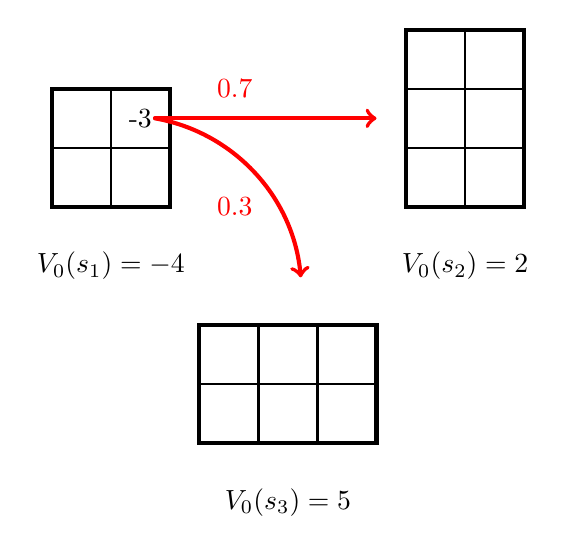
\begin{tikzpicture}[x=0.75cm,y=0.75cm]
       \draw[black, thick, line width=1.5pt, line cap=rect] (0,0) -- (0, -2);
       \draw[black, thick] (1,0) -- (1, -2);
       \draw[black, thick, line width=1.5pt, line cap=rect] (2,0) -- (2, -2);
       \draw[black, thick, line width=1.5pt, line cap=rect] (0,0) -- (2, 0);
       \draw[black, thick] (0,-1) -- (2, -1);
       \draw[black, thick, line width=1.5pt, line cap=rect] (0,-2) -- (2, -2) node[] at (1,-3) {$V_0(s_1) = -4$};
       
       \draw[red, thick, ->, line width=1.5pt, line cap=round] (1.75,-0.5) arc (80:5:3) node[] at (3.1, -2) {0.3};
       \draw[red, thick, ->, line width=1.5pt, line cap=round] (1.75,-0.5) -- (5.5, -0.5) node[] at (3.1, 0) {0.7};

       \node[] at (1.5,-0.5) {-3};    
     
       \draw[black, thick, line width=1.5pt, line cap=rect] (6,1) -- (6, -2);
       \draw[black, thick] (7,1) -- (7, -2);
       \draw[black, thick, line width=1.5pt, line cap=rect] (8,1) -- (8, -2);
       \draw[black, thick, line width=1.5pt, line cap=rect] (6,1) -- (8, 1);
       \draw[black, thick] (6,0) -- (8, 0);
       \draw[black, thick] (6,-1) -- (8, -1);
       \draw[black, thick, line width=1.5pt, line cap=rect] (6,-2) -- (8, -2)  node[] at (7,-3) {$V_0(s_2) = 2$};

       \draw[black, thick, line width=1.5pt, line cap=rect] (2.5,-4) -- (2.5, -6);
       \draw[black, thick] (3.5,-4) -- (3.5, -6);
       \draw[black, thick] (4.5,-4) -- (4.5, -6);
       \draw[black, thick, line width=1.5pt, line cap=rect] (5.5,-4) -- (5.5, -6);
       \draw[black, thick, line width=1.5pt, line cap=rect] (2.5,-4) -- (5.5, -4);
       \draw[black, thick] (2.5,-5) -- (5.5, -5);
       \draw[black, thick, line width=1.5pt, line cap=rect] (2.5,-6) -- (5.5, -6) node[] at (4,-7) {$V_0(s_3) = 5$};
      \end{tikzpicture}
     \end{center}
    \end{column}
    \begin{column}{0.3\textwidth}
     \visible<2->{\begin{center}
      \begin{gather*}
        -3 + \delta \; (0.7 \times 2 + 0.3 \times 5) \\ = -3 + 2.9 \; \delta
      \end{gather*}
      \vspace{2em}
      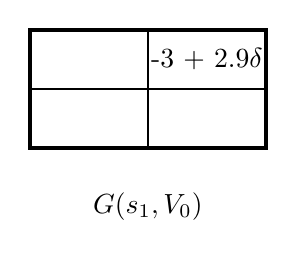
\begin{tikzpicture}[x=0.75cm,y=0.75cm]
       \draw[black, thick, line width=1.5pt, line cap=rect] (-2,0) -- (-2, -2);
       \draw[black, thick] (0,0) -- (0, -2);
       \draw[black, thick, line width=1.5pt, line cap=rect] (2,0) -- (2, -2);
       \draw[black, thick, line width=1.5pt, line cap=rect] (-2,0) -- (2, 0);
       \draw[black, thick] (-2,-1) -- (2, -1);
       \draw[black, thick, line width=1.5pt, line cap=rect] (-2,-2) -- (2, -2) node[] at (0,-3) {$G(s_1, V_0)$};
       
       \node[] at (1,-0.5) {-3 + 2.9$\delta$};
      \end{tikzpicture}
     \end{center}}
    \end{column}
   \end{columns}
  \end{frame}
  
  
  \begin{frame}{Pollatschek \& Avi-Itzhak Algorithm (Extension of Policy Iteration)}
   \begin{algorithm*}[H]
    Initialize $V(s)$ arbitrarily for all $s$\Comment*{Agent 1's utility for being in $s$}
    \Repeat{until $\pi_1(s)$ and $\pi_2(s)$ converge for all $s$}{
     \For{each state $s$}{
      Compute matrix game $G(s,V)$ as in Shapley's algorithm\;
      $\pi_1(s)$ $\leftarrow$ maxmin strategy of Agent 1 in $G(s,V)$\;
      $\pi_2(s)$ $\leftarrow$ minmax strategy agents Agent 1 in $G(s,V)$\;
     }
     
     Calculate $V(s)$ with policy evaluation for $\pi_1$ and $\pi_2$
    }
   \end{algorithm*}
  \end{frame}
  
  
  \begin{frame}{Acknowledgment}
   \begin{itemize}
   \setlength{\itemsep}{1em}
    \item This lecture is a slightly modified version of ones prepared by
    \begin{itemize}
     \item Dan Klein and Pieter Abbeel \href{http://ai.berkeley.edu/home.html}{[UC Berkeley CS 188]}
     \item Vincent Conitzer \href{https://courses.cs.duke.edu/spring16/compsci590.4/}{[Duke CPS 590.4]}
    \end{itemize}
   \end{itemize}
  \end{frame}



\end{document}
